% Committee progress review, 23 September 2026.
% Audience: thesis committee, most of whom have not followed the work.
% Register deliberately differs from the minor report: no repository paths on
% slides, findings ordered by research question rather than by campaign.
\documentclass[aspectratio=169,11pt]{beamer}

\usetheme{metropolis}
\usepackage[T1]{fontenc}
\usepackage[utf8]{inputenc}
\usepackage{booktabs}
\usepackage{siunitx}
\usepackage{graphicx}
\usepackage{tikz}
\usetikzlibrary{arrows.meta,fit,positioning,shapes.geometric}
\usepackage{xcolor}

% Status colours shared with the minor report's architecture figure.
\definecolor{implemented}{HTML}{D9EAD3}
\definecolor{external}{HTML}{D9EAF7}
\definecolor{blocked}{HTML}{F4CCCC}
\definecolor{planned}{HTML}{FFF2CC}
\definecolor{flagred}{HTML}{B00000}
\newcommand{\code}[1]{\texttt{\small #1}}
\newcommand{\bad}[1]{\textcolor{flagred}{#1}}

\setbeamertemplate{caption}{\raggedright\insertcaption\par}
\metroset{block=fill}

\title{Vision-Based Navigation for AMRs\\in a Dynamic Warehouse}
\subtitle{Progress review}
\author{Bolton Athit Davies}
\date{23 September 2026}

\begin{document}

\maketitle

% ---------------------------------------------------------------- question
\begin{frame}{The question}
  Can a vision-based pipeline provide reliable localization for an autonomous
  mobile robot in a warehouse \emph{that contains moving objects}?

  \vspace{1em}
  Two sub-questions:
  \begin{enumerate}
    \item How do the two leading stereo-inertial pipelines --- ORB-SLAM3 and
      VINS-Fusion --- behave under controlled changes in scene dynamics, floor
      texture and compute load?
    \item Does masking dynamic objects with a learned detector improve
      localization, and by how much?
  \end{enumerate}

  \vspace{1em}
  \alert{Path planning is outside the scope.} The deliverable is a reliable
  navigation state and map, not a planner.
\end{frame}

\begin{frame}{What exists at the cutoff}
  \centering
  \resizebox{0.80\textwidth}{!}{% Experimental architecture. Nodes are placed on an explicit grid rather than by
% relative chaining: the detector sits between the two estimators so that its two
% optional edges are short verticals instead of connectors routed through the
% estimator boxes, and every arrow enters a distinct face of its target node.
% The trajectory-to-RTAB-Map gap is sized to hold its edge label clear of both
% boxes and of the grouping rectangle.
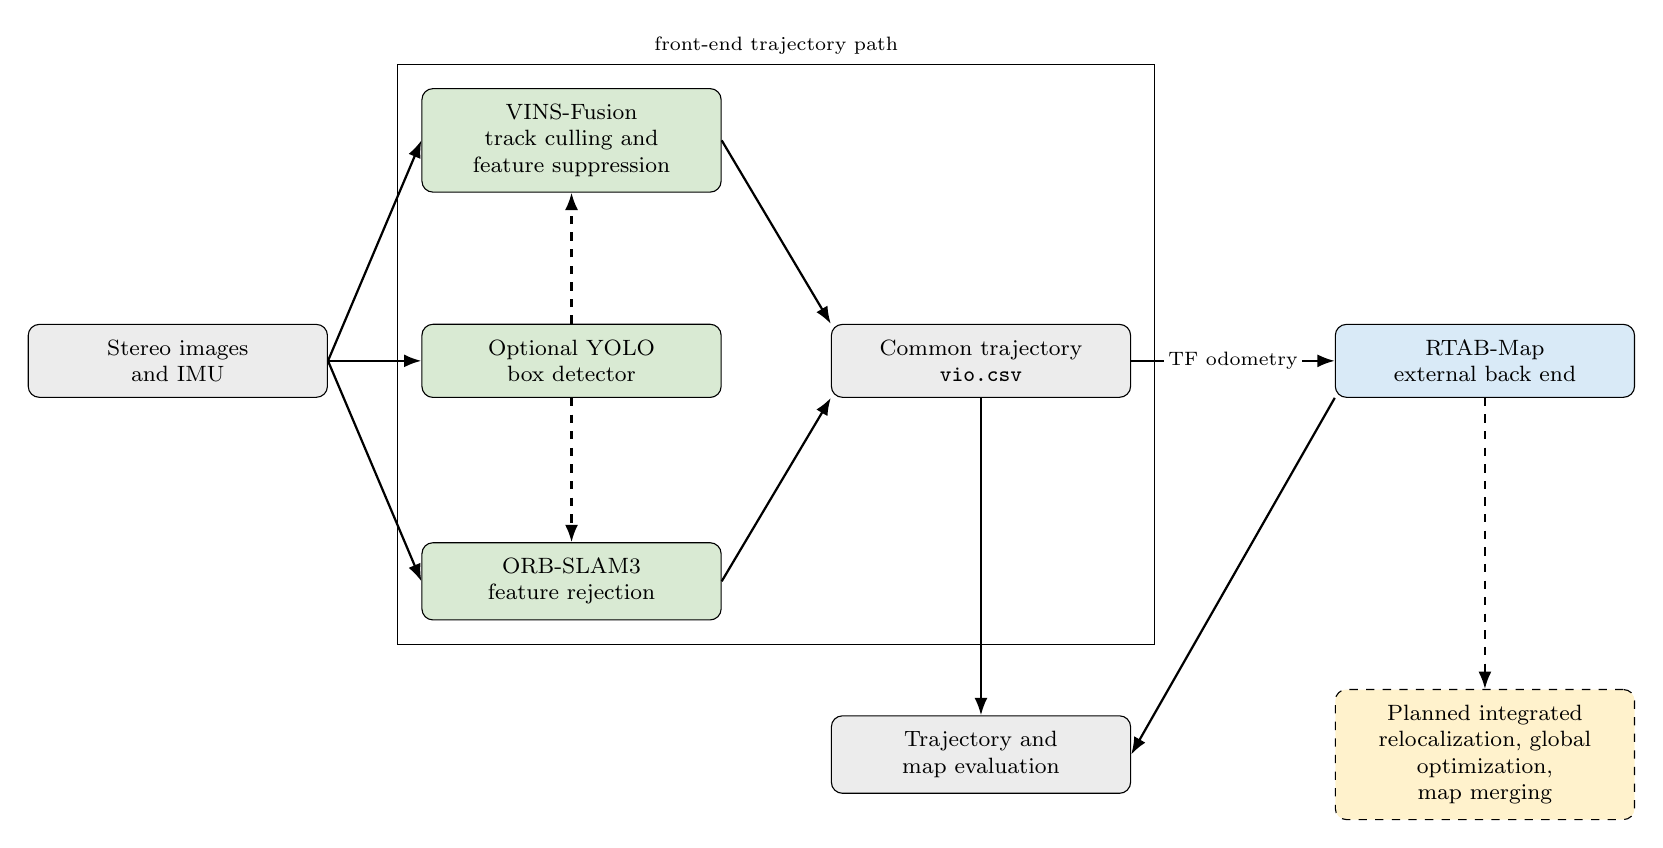
\begin{tikzpicture}[
  block/.style={draw, rounded corners, align=center, minimum height=9mm,
    text width=34mm, font=\footnotesize, fill=implemented, inner sep=2mm},
  source/.style={block, fill=gray!15},
  backend/.style={block, fill=external},
  plan/.style={block, fill=planned, dashed},
  flow/.style={-{Latex[length=2.2mm]}, thick},
  optional/.style={flow, dashed},
  edgelabel/.style={font=\scriptsize, fill=white, inner sep=1.5pt}
]
  \node[source]  at ( 0.0,  0.0) (sensors)    {Stereo images\\and IMU};
  \node[block]   at ( 5.0,  2.8) (vins)       {VINS-Fusion\\track culling and\\feature suppression};
  \node[block]   at ( 5.0,  0.0) (detector)   {Optional YOLO\\box detector};
  \node[block]   at ( 5.0, -2.8) (orb)        {ORB-SLAM3\\feature rejection};
  \node[source]  at (10.2,  0.0) (trajectory) {Common trajectory\\\texttt{vio.csv}};
  \node[backend] at (16.6,  0.0) (rtab)       {RTAB-Map\\external back end};
  \node[source]  at (10.2, -5.0) (evaluation) {Trajectory and\\map evaluation};
  \node[plan]    at (16.6, -5.0) (future)     {Planned integrated\\relocalization, global\\optimization, map merging};

  % Sensor stream reaches the detector and both estimators without crossings.
  \draw[flow] (sensors.east) -- (vins.west);
  \draw[flow] (sensors.east) -- (detector.west);
  \draw[flow] (sensors.east) -- (orb.west);

  % Optional masks: short verticals, so nothing is drawn across a box.
  \draw[optional] (detector.north) -- (vins.south);
  \draw[optional] (detector.south) -- (orb.north);

  % Both estimators write the common trajectory; they enter the two left corners
  % so the arrowheads stay apart and the south face is free for the next edge.
  \draw[flow] (vins.east) -- (trajectory.north west);
  \draw[flow] (orb.east) -- (trajectory.south west);
  \draw[flow] (trajectory.south) -- (evaluation.north);
  \draw[flow] (trajectory.east) -- node[edgelabel]{TF odometry} (rtab.west);
  \draw[flow] (rtab.south west) -- (evaluation.east);
  \draw[optional] (rtab.south) -- (future.north);

  \node[draw, fit=(vins)(orb)(trajectory), inner sep=3mm,
    label={[font=\scriptsize]above:front-end trajectory path}] {};
\end{tikzpicture}
}

  \vspace{0.3em}
  \footnotesize Green: built here. Blue: external. Dashed yellow: future work.
  There is deliberately \emph{no} feedback arrow from RTAB-Map into either front
  end.
\end{frame}

% ---------------------------------------------------------------- method
\begin{frame}{The methodological core: admissibility before results}
  Every comparison is tested for validity \emph{before} its numbers are read.
  A run is descriptive unless it passes:

  \vspace{0.8em}
  \begin{itemize}
    \item same recorded input to both treatments, within \SI{5}{\percent} on
      frame count and duration;
    \item the intended treatment demonstrably active, not merely requested;
    \item a common ground-truth interval, with the matched sample count reported;
    \item physical plausibility --- no step implying more than
      \SI{10}{\metre\per\second}.
  \end{itemize}

  \vspace{0.8em}
  This protocol is what produced most of the findings in this review, including
  two that would otherwise have entered the thesis as results.
\end{frame}

% ---------------------------------------------------------------- headline
\begin{frame}{Finding 1: the dead-reckoning floor is higher than expected}
  Five recordings, four worlds, all five estimators on identical data.
  Aligned ATE RMSE in metres.

  \vspace{0.5em}
  \centering\small
  \begin{tabular}{lrrrrr}
    \toprule
    Dataset & IMU only & Wheel & VINS & ORB & \textbf{EKF} \\
    \midrule
    \code{allsensor\_000} & 21.70 & 2.80 & 0.62 & 0.58 & \textbf{0.19} \\
    \code{allsensor\_001} & 12.62 & 0.98 & 0.38 & 0.37 & \textbf{0.31} \\
    \code{allsensor\_002} & 13.24 & 1.49 & 0.56 & 0.60 & \textbf{0.26} \\
    \code{allsensor\_003} & 45.56 & 3.19 & 0.78 & \bad{6.48} & \textbf{0.42} \\
    \code{allsensor\_004} & 26.71 & 3.24 & \textbf{0.43} & 1.24 & 0.49 \\
    \bottomrule
  \end{tabular}

  \vspace{0.8em}
  \begin{alertblock}{}
    A wheel+IMU EKF beats both visual pipelines on four of five datasets, at
    \SIrange{0.10}{0.88}{\percent} drift. \textbf{In static scenes the visual
    pipeline does not yet earn its keep.}
  \end{alertblock}
\end{frame}

\begin{frame}{Why that finding matters}
  It is not a negative result about the method --- it is the missing baseline.

  \vspace{1em}
  \begin{itemize}
    \item Before this, every trajectory figure reported visual error against
      ground truth \emph{with nothing to compare it to}.
    \item Four hypotheses were registered before the metrics were computed. One
      was falsified by its own data.
    \item The EKF's advantage is specific to these conditions: static scene,
      perfect wheel encoders, no slip. It is a floor the visual system must
      clear, not a replacement for it.
  \end{itemize}

  \vspace{1em}
  The honest reading: \textbf{vision must justify itself where dead reckoning
  fails} --- long runs, wheel slip, relocalization after loss, and dynamic
  scenes.
\end{frame}

% ---------------------------------------------------------------- other findings
\begin{frame}{Finding 2: the detector's limit is detection, not semantics}
  \SI{9860}{} camera frames, ground truth projected from simulator object poses.

  \vspace{0.8em}
  \begin{columns}[T]
    \begin{column}{0.48\textwidth}
      \metroset{block=fill}
      \begin{block}{Bounding-box detection}
        precision \textbf{0.684}\\
        recall \textbf{0.593}\\
        moving-object recall \textbf{0.591}
      \end{block}
    \end{column}
    \begin{column}{0.48\textwidth}
      \begin{block}{Class, once localized}
        accuracy \textbf{0.996}\\
        \SI{37061}{} associated objects\\
        137 substitutions
      \end{block}
    \end{column}
  \end{columns}

  \vspace{0.8em}
  The model names objects almost perfectly once it finds them, and misses about
  \SI{41}{\percent} of the moving ones. Improving the classifier would change
  nothing; \textbf{recall is the binding constraint}.

  \vspace{0.5em}
  \footnotesize Also: the detector outputs boxes, not segmentation, and class
  membership is not evidence of motion. There is no 3-D motion gate.
\end{frame}

\begin{frame}{Finding 3: the reconstructed map is geometrically sound}
  Tiny warehouse, RTAB-Map database scored against the simulator's own collision
  geometry at \SI{0.25}{\metre} tolerance.

  \vspace{0.8em}
  \centering
  \begin{tabular}{lr}
    \toprule
    Occupied-cell precision & \textbf{\SI{96.6}{\percent}} \\
    Recall, region observed & \SI{89.5}{\percent} \\
    Recall, whole building & \SI{67.2}{\percent} \\
    \bottomrule
  \end{tabular}

  \vspace{0.8em}
  \raggedright
  The gap between \SI{89.5}{} and \SI{67.2}{\percent} is route coverage, not
  mapping failure: the run never entered the side aisles.

  \vspace{0.5em}
  \footnotesize The drivability half of this evaluation was found to be scored
  against the run that \emph{built} the map. Caught by comparing node poses
  against ground truth at matching timestamps; reported as queried rather than
  used.
\end{frame}

\begin{frame}{Finding 4: neither pipeline runs at input rate}
  Frames arrive every \SI{33}{\milli\second}. Median per-stage cost:

  \vspace{0.8em}
  \centering\small
  \begin{tabular}{lrr}
    \toprule
    & Without detector & With detector \\
    \midrule
    ORB-SLAM3 tracking & \SI{63}{\milli\second} & \SI{113}{\milli\second} \\
    ORB-SLAM3 local mapping & \SI{190}{\milli\second} & \SI{356}{\milli\second} \\
    VINS-Fusion back end & \SI{60}{\milli\second} & --- \\
    \midrule
    Input retained & \SI{89}{\percent} & \SI{67}{\percent} \\
    \bottomrule
  \end{tabular}

  \vspace{0.8em}
  \raggedright
  ORB-SLAM3 discards frames at its own subscriber under load; VINS-Fusion
  buffers them. \textbf{The two differ in queue policy as well as algorithm}, so
  throughput is not yet a fair comparison between them.
\end{frame}

% ---------------------------------------------------------------- problems
\begin{frame}{Withheld: the dynamic-scene results}
  The dynamic worlds are \textbf{not yet a physical simulation}. Props follow
  scripted kinematic paths: collision geometry, but no dynamic response against
  the robot and no constraint to behave as warehouse traffic would.

  \vspace{0.6em}
  \begin{alertblock}{}
    48 runs logged, all 48 fail the plausibility check --- and they are
    \textbf{withheld, not reported as findings}. They describe the simulation,
    not the problem.
  \end{alertblock}

  \vspace{0.6em}
  \raggedright
  A scoping decision, not a failure to measure --- the runs stay in the record as
  excluded evidence. Two consequences: the condition this thesis is named for has
  \textbf{no valid testbed yet}, untested rather than tested and failed; and the
  environment becomes the leading candidate cause of the breakdown, as well as
  the cheapest to test.
\end{frame}

\begin{frame}{What is \emph{not} established: the core hypothesis}
  Semantic filtering --- the contribution the thesis is named for --- has
  \textbf{no valid test behind it yet}. Two instrumentation faults:

  \vspace{1em}
  \begin{itemize}
    \item \textbf{The VINS filter never fired.} All 12 runs requested it; all 12
      record zero matched detector frames, zero mask coverage, zero removed
      tracks. The detector works offline --- the masks never reached the tracker.
    \item \textbf{ORB pairs were not paired.} 11 of 12 baseline/filtered pairs
      received frame counts differing by \SIrange{10}{30}{\percent} on the same
      recording, while durations matched to \SI{0.13}{\percent}.
  \end{itemize}

  \vspace{1em}
  Both were caught by the admissibility protocol, \textbf{before} any
  filter-versus-baseline number was reported. One valid pair exists out of
  twenty-four.

  \vspace{0.6em}
  These are faults in the code path, so they stand regardless of the scene. But
  the filtered runs were recorded in the dynamic worlds --- so once those are
  withheld, the hypothesis needs \textbf{both} a working mask path and a valid
  environment to be tested in.
\end{frame}

\begin{frame}{The audit is the result}
  Four claims were retracted or prevented this period:

  \vspace{0.8em}
  \begin{enumerate}
    \item A camera-rotation parsing bug that made the map a smear --- found by
      map distortion, not by ATE, which looked plausible throughout.
    \item A map judged ``not navigable'' --- the grid had been mis-seated, so
      real structure was scored against the wrong cells.
    \item A drivability score measured against the map's own construction run.
    \item The two filter faults above.
  \end{enumerate}

  \vspace{0.8em}
  \begin{block}{}
    Every one of these would have entered the thesis as a result. The protocol
    that catches them is, at this stage, the most transferable output of the
    work.
  \end{block}
\end{frame}

% ---------------------------------------------------------------- plan
\begin{frame}{Next period}
  \small
  \begin{tabular}{llp{5.2cm}}
    \toprule
    Priority & Action & Unblocks \\
    \midrule
    1 & Rebuild the dynamic worlds with physically simulated props & Gives the
      thesis's titular condition a valid testbed. Also the cheapest candidate
      cause for the breakdown. \\
    2 & Fix the VINS mask delivery path & The core hypothesis, on the code side.
      Needs no new data. \\
    3 & Equalise ORB input across paired runs & Makes the filter comparison
      admissible. \\
    4 & Add disturbance to the simulation & Wheel slip and encoder quantisation;
      both idealisations currently favour the dead-reckoning baseline. \\
    5 & Independent route for map drivability & One new recording, not a new
      map. \\
    6 & Large-warehouse map evaluation & Extends map results beyond the tiny
      world. \\
    \bottomrule
  \end{tabular}
\end{frame}

\begin{frame}{Where I need the committee's guidance}
  \begin{enumerate}
    \item \textbf{Scope.} Given that a wheel+IMU EKF currently beats both visual
      pipelines in static scenes, should the thesis argue for vision as the
      primary sensor, or reframe around \emph{when} vision adds value over dead
      reckoning?

      \vspace{0.6em}
    \item \textbf{Depth versus breadth.} Rebuild the dynamic environment
      properly before measuring anything further in it, or broaden to the real
      robot and the large warehouse with the static results as they stand?

      \vspace{0.6em}
    \item \textbf{The integration direction.} Relocalization, global
      optimization and map merging are listed as future work. Is that the right
      next contribution, or a distraction until dynamic-scene tracking is sound?
  \end{enumerate}
\end{frame}

\begin{frame}[standout]
  Questions
\end{frame}

% ---------------------------------------------------------------- backup
\appendix

\begin{frame}{Backup: static-scene repeatability}
  Three static datasets, three repeats each, median (IQR).

  \vspace{0.8em}
  \centering
  \begin{tabular}{lrr}
    \toprule
    & Translational ATE & Rotational RMSE \\
    \midrule
    VINS-Fusion & \SI{0.370}{\metre} (0.063) & \SI{1.56}{\degree} (0.98) \\
    ORB-SLAM3 & \SI{0.454}{\metre} (0.157) & \SI{17.92}{\degree} (1.72) \\
    \bottomrule
  \end{tabular}

  \vspace{0.8em}
  \raggedright
  Positional error is comparable; rotational error differs elevenfold. But
  jump-free rotational RPE is \SIrange{0.10}{0.66}{\degree} for ORB-SLAM3 against
  \SIrange{0.49}{0.69}{\degree} for VINS-Fusion. \textbf{The entire gap comes from
  one or two discrete events per run}, not from worse orientation tracking.
\end{frame}

\begin{frame}{Backup: evidence base}
  \begin{itemize}
    \item 66 logged estimator runs across seven simulation datasets, three
      repeats per condition.
    \item Five multi-sensor recordings spanning four worlds, used for the
      baseline comparison.
    \item \SI{9860}{} camera frames with projected object ground truth.
    \item One RTAB-Map database with graph, geometry and drivability evaluation.
    \item Per-frame timing, delivery, CPU and memory records for every run.
  \end{itemize}

  \vspace{1em}
  Full detail, including all retracted and excluded measurements, is in the
  accompanying progress report.
\end{frame}

\end{document}
